\section{Experimental Results}
\label{sec:exp}

In this section, we conduct experiments on a synthetic data set and a real data set 
to verify the effectiveness of our proposed worker model and debiasing technique.  

\vpara{Data sets.}
We first introdue the data sets we used in this experiments.  


\begin{figure}[!t]
  \centering
  \subfigure[Parameter analysis]{
    \label{subfig:beta}
    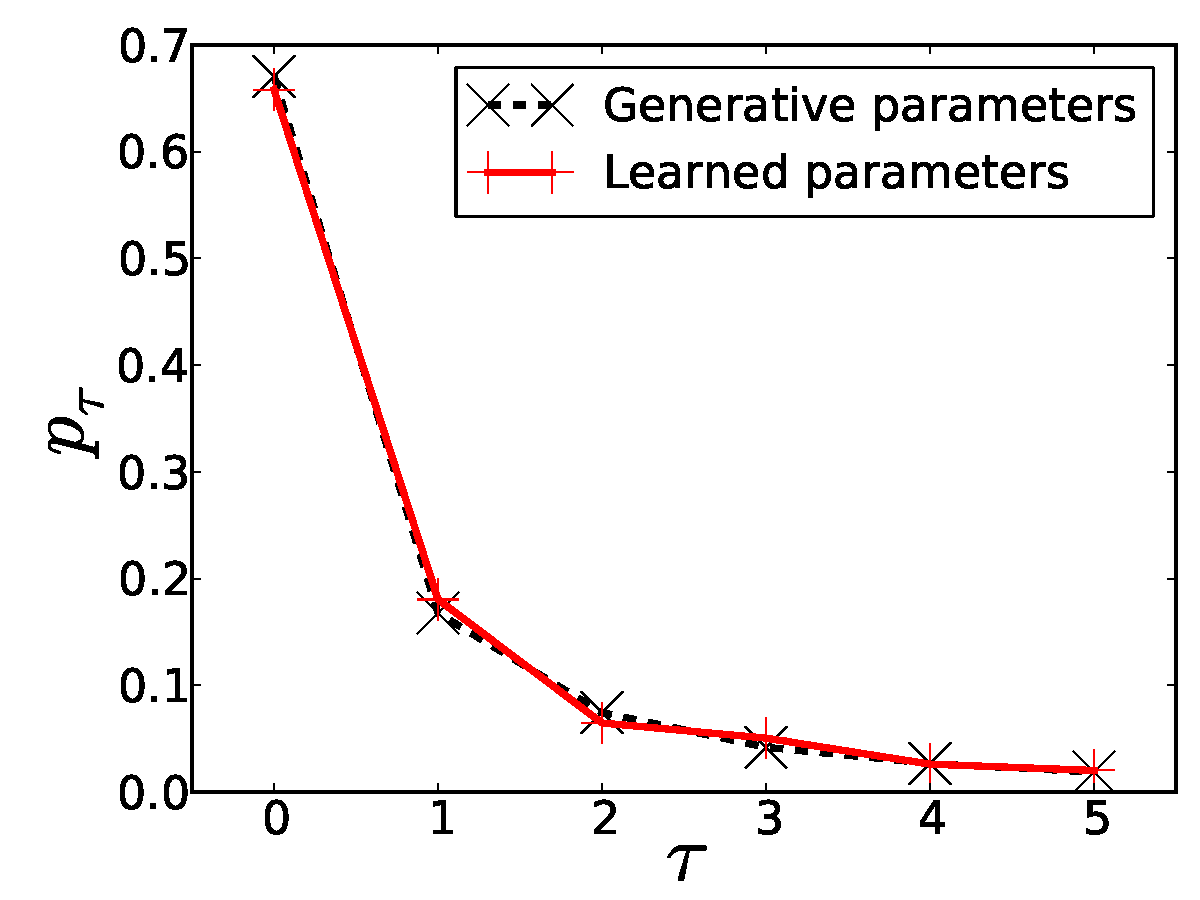
\includegraphics[width=0.46\columnwidth]{figures/ptau_synthetic}
  }
  \subfigure[Convergence analysis]{
    \label{subfig:convergence}
    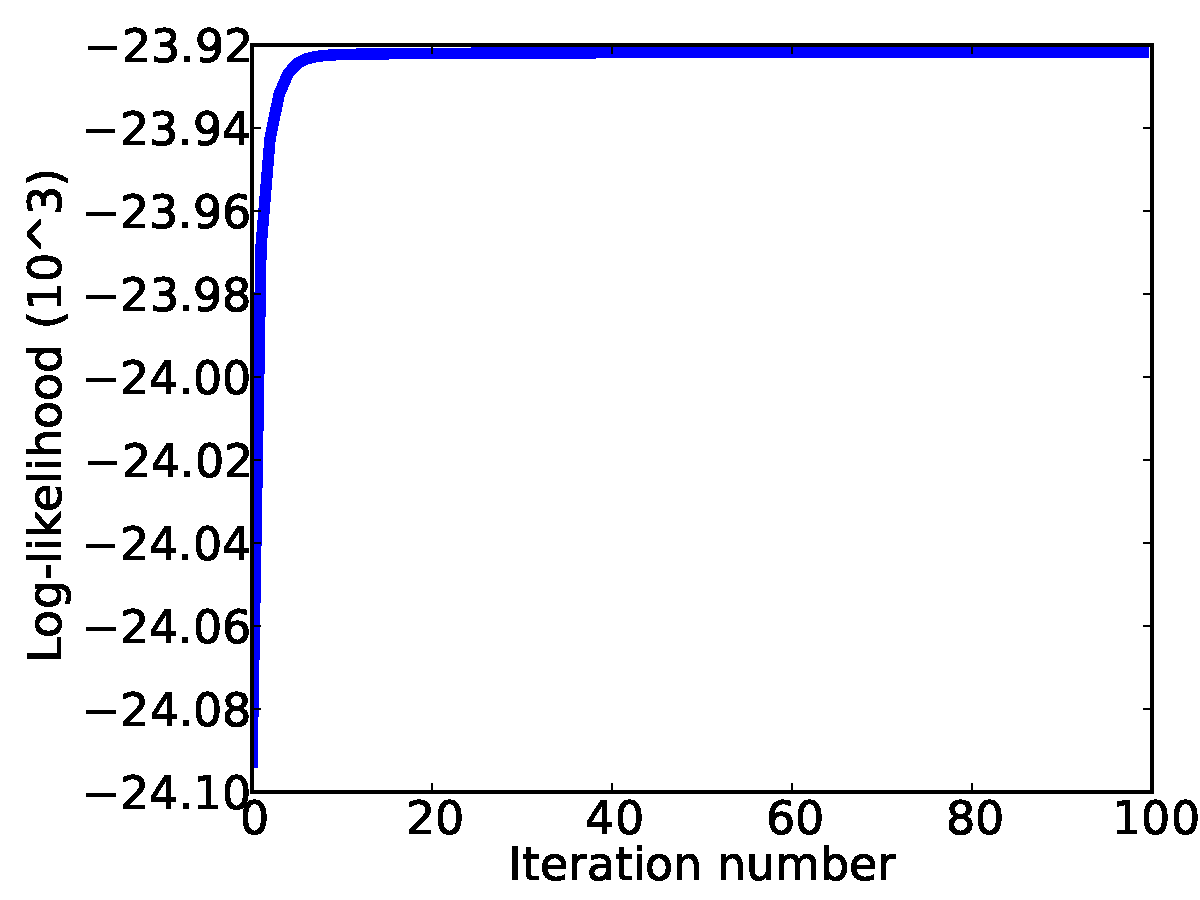
\includegraphics[width=0.46\columnwidth]{figures/loglikelihood_synthetic}
  }
  \caption{\label{fig:modelanalysis}Factor graph model parameter and convergence
    results when trained to characterize in-batch bias in crowdsourced annotation.
  }
\end{figure}

\begin{figure}[!t]
  \centering
  \subfigure[Parameter analysis]{
    \label{subfig:beta}
    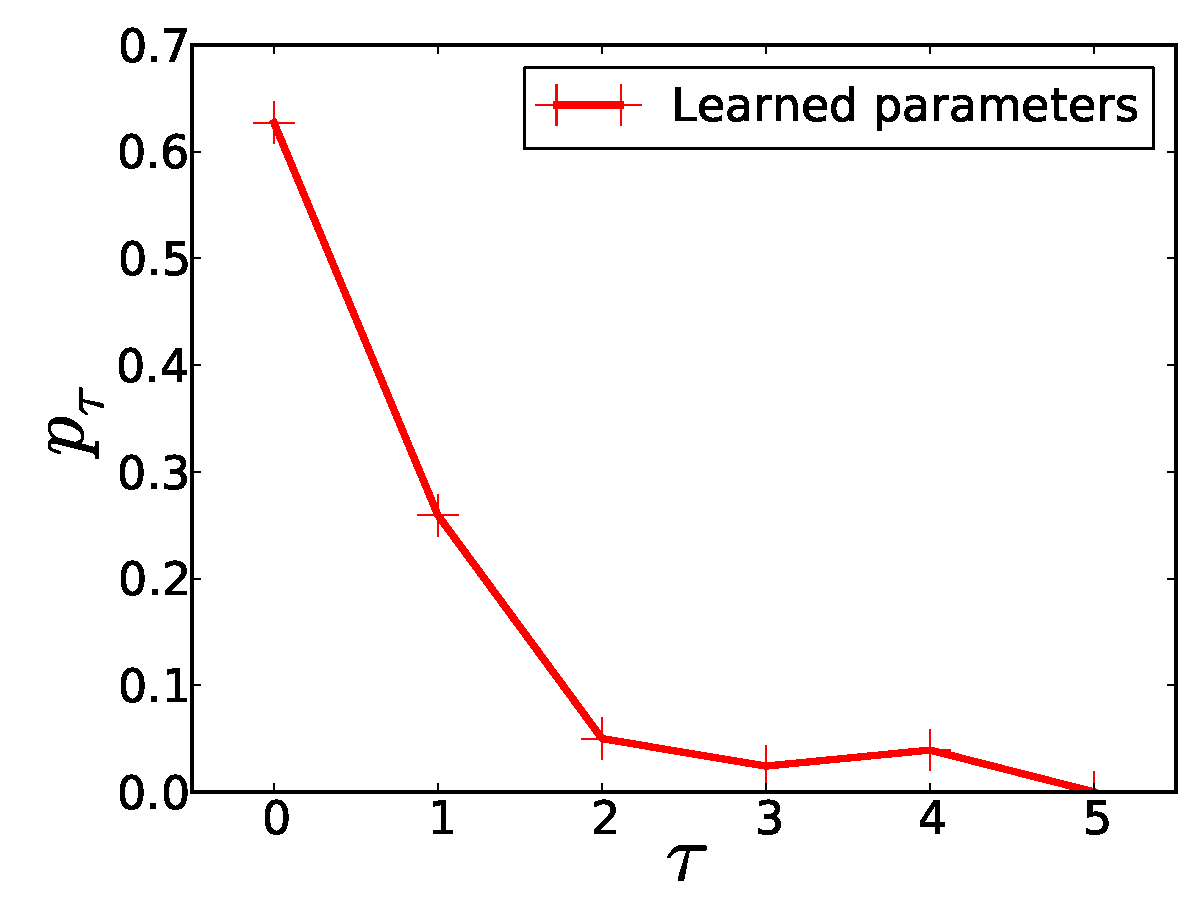
\includegraphics[width=0.46\columnwidth]{figures/ptau_lnkd}
  }
  \subfigure[Convergence analysis]{
    \label{subfig:convergence}
    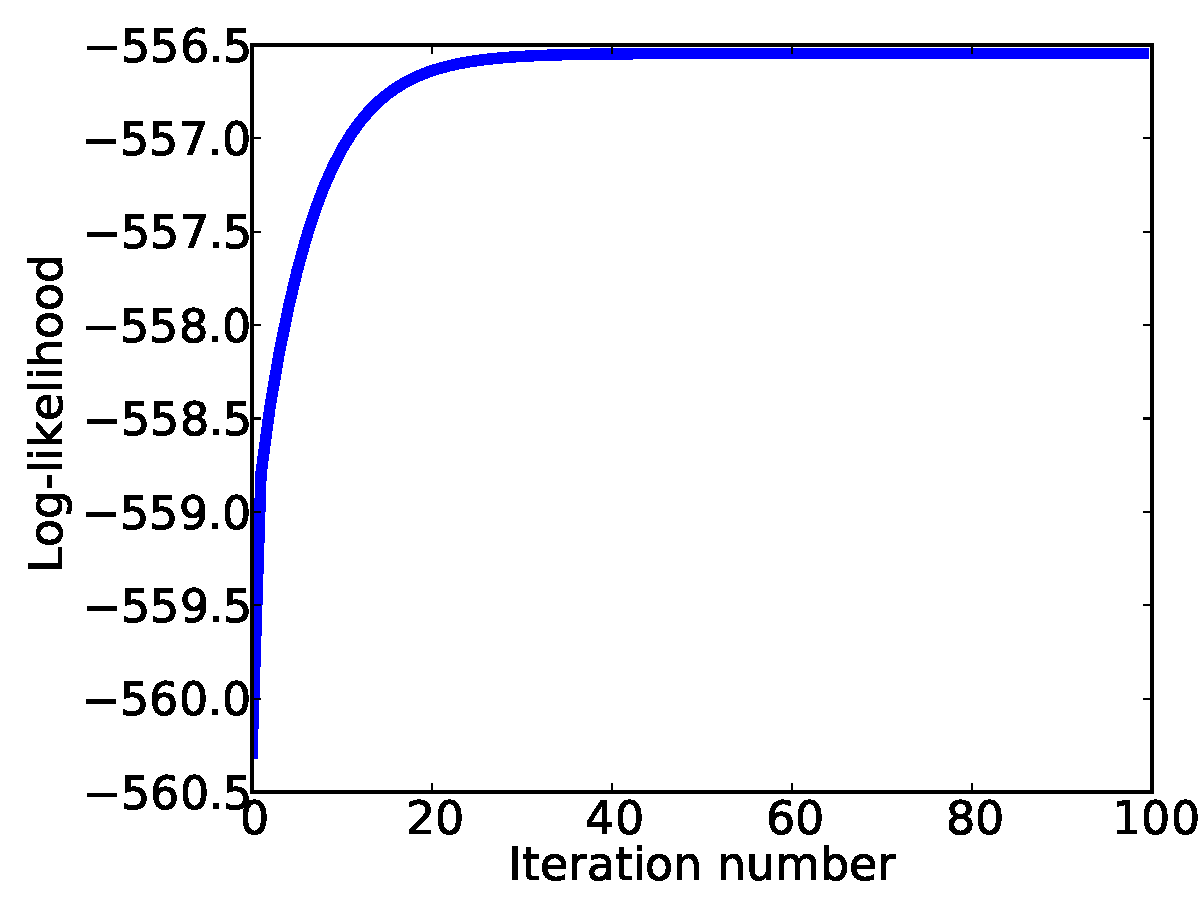
\includegraphics[width=0.46\columnwidth]{figures/loglikelihood_lnkd}
  }
  \caption{\label{fig:modelanalysis}Factor graph model parameter and convergence
    results when trained to characterize in-batch bias in crowdsourced annotation.
  }
\end{figure}